%%%%%%%%%%%%%%%%%%%%%%%%%%%%%%%%%%%%%%%%%
% Beamer Presentation
% LaTeX Template
% Version 1.0 (10/11/12)
%
% This template has been downloaded from:
% http://www.LaTeXTemplates.com
%
% License:
% CC BY-NC-SA 3.0 (http://creativecommons.org/licenses/by-nc-sa/3.0/)
%
%%%%%%%%%%%%%%%%%%%%%%%%%%%%%%%%%%%%%%%%%

%----------------------------------------------------------------------------------------
%	PACKAGES AND THEMES
%----------------------------------------------------------------------------------------

\documentclass[11pt]{beamer}

\mode<presentation> {

% The Beamer class comes with a number of default slide themes
% which change the colors and layouts of slides. Below this is a list
% of all the themes, uncomment each in turn to see what they look like.

%\usetheme{default}
%\usetheme{AnnArbor}
%\usetheme{Antibes}
%\usetheme{Bergen}
%\usetheme{Berkeley}
%\usetheme{Berlin}
%\usetheme{Boadilla}
\usetheme{CambridgeUS}
%\usetheme{Copenhagen}
%\usetheme{Darmstadt}
%\usetheme{Dresden}
%\usetheme{Frankfurt}
%\usetheme{Goettingen}
%\usetheme{Hannover}
%\usetheme{Ilmenau}
%\usetheme{JuanLesPins}
%\usetheme{Luebeck}
%\usetheme{Madrid}
%\usetheme{Malmoe}
%\usetheme{Marburg}
%\usetheme{Montpellier}
%\usetheme{PaloAlto}
%\usetheme{Pittsburgh}
%\usetheme{Rochester}
%\usetheme{Singapore}
%\usetheme{Szeged}
%\usetheme{Warsaw}

% As well as themes, the Beamer class has a number of color themes
% for any slide theme. Uncomment each of these in turn to see how it
% changes the colors of your current slide theme.

%\usecolortheme{albatross}
%\usecolortheme{beaver}
%\usecolortheme{beetle}
%\usecolortheme{crane}
\usecolortheme{dolphin}
%\usecolortheme{dove}
%\usecolortheme{fly}
%\usecolortheme{lily}
%\usecolortheme{orchid}
%\usecolortheme{rose}
%\usecolortheme{seagull}
%\usecolortheme{seahorse}
%\usecolortheme{whale}
%\usecolortheme{wolverine}

%\setbeamertemplate{footline} % To remove the footer line in all slides uncomment this line
%\setbeamertemplate{footline}[page number] % To replace the footer line in all slides with a simple slide count uncomment this line

%\setbeamertemplate{navigation symbols}{} % To remove the navigation symbols from the bottom of all slides uncomment this line
}
%\usepackage[]{mcode}
\usepackage{gensymb}
\usepackage{alltt}
\usepackage{amsmath}
\usepackage{graphicx} % Allows including images
\usepackage{booktabs} % Allows the use of \toprule, \midrule and \bottomrule in tables
\usepackage[font=scriptsize,labelfont=bf]{caption}
\usepackage[round]{natbib}
\usepackage[dutch]{babel}
\usepackage{xcolor}
\usepackage{tikz}
\usepackage[utf8]{inputenc} 
\usepackage{amsmath,tkz-base} 
\usetikzlibrary{matrix, fit,calc,positioning,decorations.pathreplacing}
\usepackage{textcomp}
\usepackage{microtype}
\usepackage{amsmath,tkz-base}
\usepackage{multicol}
\usepackage{pst-plot}
\newcommand\Wider[2][3em]{%
\makebox[\linewidth][c]{%
  \begin{minipage}{\dimexpr\textwidth+#1\relax}
  \raggedright#2
  \end{minipage}%
  }%
}

\usepackage{pst-plot}
\usetikzlibrary{matrix, fit,calc,positioning,decorations.pathreplacing}
\setbeamerfont{block body}{size=\small}
\bibliographystyle{plainnat}
\nocite{*}
%----------------------------------------------------------------------------------------
%	TITLE PAGE
%----------------------------------------------------------------------------------------

\title[Predicting pathogen invasion]{Predicting pathogen invasion in synthetic communities in function of evenness} % The short title appears at the bottom of every slide, the full title is only on the title page

\author{Wai Kit Tsang} % Your name

\institute[LabMET \& KERMIT] % Your institution as it will appear on the bottom of every slide, may be shorthand to save space
{

%\centering
\begin{tabular}{l l }
Promotors: & Prof. dr. ir. Nico Boon \\
		   & Prof. dr. Willem Waegeman \\
Tutor: 	   & Ir. Michiel Stock \\
    	   & Dr. Ramiro V\'ilchez Vargas \\
%Tutors: 	   & Dr. Ramiro V\'ilchez Vargas \\
%    	   & Ir. Michiel Stock \\    	   
\end{tabular}

%Promotors: Prof. dr. ir. Nico Boon \&  \\ Prof. dr. Willem Waegeman \\ tutor: dr. Ramiro V\'ilchez Vargas \& ir. Michiel Stock \\
\medskip
Ghent University \\ % Your institution for the title page
\medskip
\textit{waikit.tsang@ugent.be} % Your email address
}
\date{\today} % Date, can be changed to a custom date

\begin{document}

\begin{frame}
\titlepage % Print the title page as the first slide
\end{frame}

%----------------------------------------------------------------------------------------
%	PRESENTATION SLIDES
%----------------------------------------------------------------------------------------

%------------------------------------------------
%\section{Introduction} % Sections can be created in order to organize your presentation into discrete blocks, all sections and subsections are automatically printed in the table of contents as an overview of the talk
%------------------------------------------------

%\subsection{Wet Lab Experiments vs In silico Prediction} % A subsection can be created just before a set of slides with a common theme to further break down your presentation into chunks

\begin{frame}
\frametitle{Background}
\setbeamercolor{block title}{use=structure,fg=white,bg=blue!75!black}
\setbeamercolor{block body}{use=structure,fg=black,bg=white!20!white}

\textbf{Motivation}\\
Gathering my own data and machine learning to predict pathogen invasion. \\
\medskip
\textbf{Microbial aspect}\\
\begin{itemize}
\item Initial community evenness favours functionality under selective stress. \citep{wittebolle2009initial}
\item Evenness describes the relative abundance of species in a community.
\item How does the initial community evenness influence pathogen invasion in a community?
\end{itemize}

\begin{block}{Definition Pielou's Evenness}
$$
J' = \displaystyle\frac{-\sum_{i = 1}^{N}p_i\ln{p_i}}{ln(N)}
$$
\end{block}

\end{frame}

\begin{frame}
\setbeamercolor{block title}{use=structure,fg=white,bg=blue!75!black}
\setbeamercolor{block body}{use=structure,fg=black,bg=white!20!white}
\frametitle{Aim}
\begin{block}{To reject Null hypothesis}
$
H_0: \mathcal{P(} \text{Invasion} \cap \text{evenness = High)} =\mathcal{P(} \text{Invasion} \cap \text{evenness = Low)}
$
\end{block}
\vspace*{.05in}
Ideally a 2-factor design tests for this hypothesis.

\begin{columns}[c] % The "c" option specifies centered vertical alignment while the "t" option is used for top vertical alignment

\column{.3\textwidth} % Left column and width
\begingroup
    \fontsize{10pt}{12pt}\selectfont
  \includegraphics[scale = .15]{finalplot.png}

\endgroup
\column{.5\textwidth} % Right column and width

\textbf{Synthetic community}
\begin{itemize}
\item 10 bacteria in each community, in different quantitities \\(Ehsani, E.)
\item Introduce one  pathogen
\item 194 communities in entire design
\end{itemize}

\end{columns}
\end{frame}

\begin{frame}
\frametitle{Plan of the experiments}
\textbf{Preparatory work}\\

\begin{itemize}
\item All 194 communities are prepared in advance and frozen in cryovials. 
\item A selection of pathogen are made strepto- and spectinomycin resistant.
\item Pathogen are frozen in the freezer.
\end{itemize}

\textbf{Actual experiment}
\begin{itemize}
\item Pull communities out of freezer and introduce one pathogen.
\item After 48 hours plate community on agar with antibiotics.
\item 48 hours after plating count the colonies
\end{itemize}
\end{frame}

\begin{frame}
\frametitle{Preparing and freezing cultures}
% Make margins wider for this slide 
\Wider[1em]{

\begin{tikzpicture}
    \node[inner sep=0pt] (incubator) at (0,4.5)
    	{ 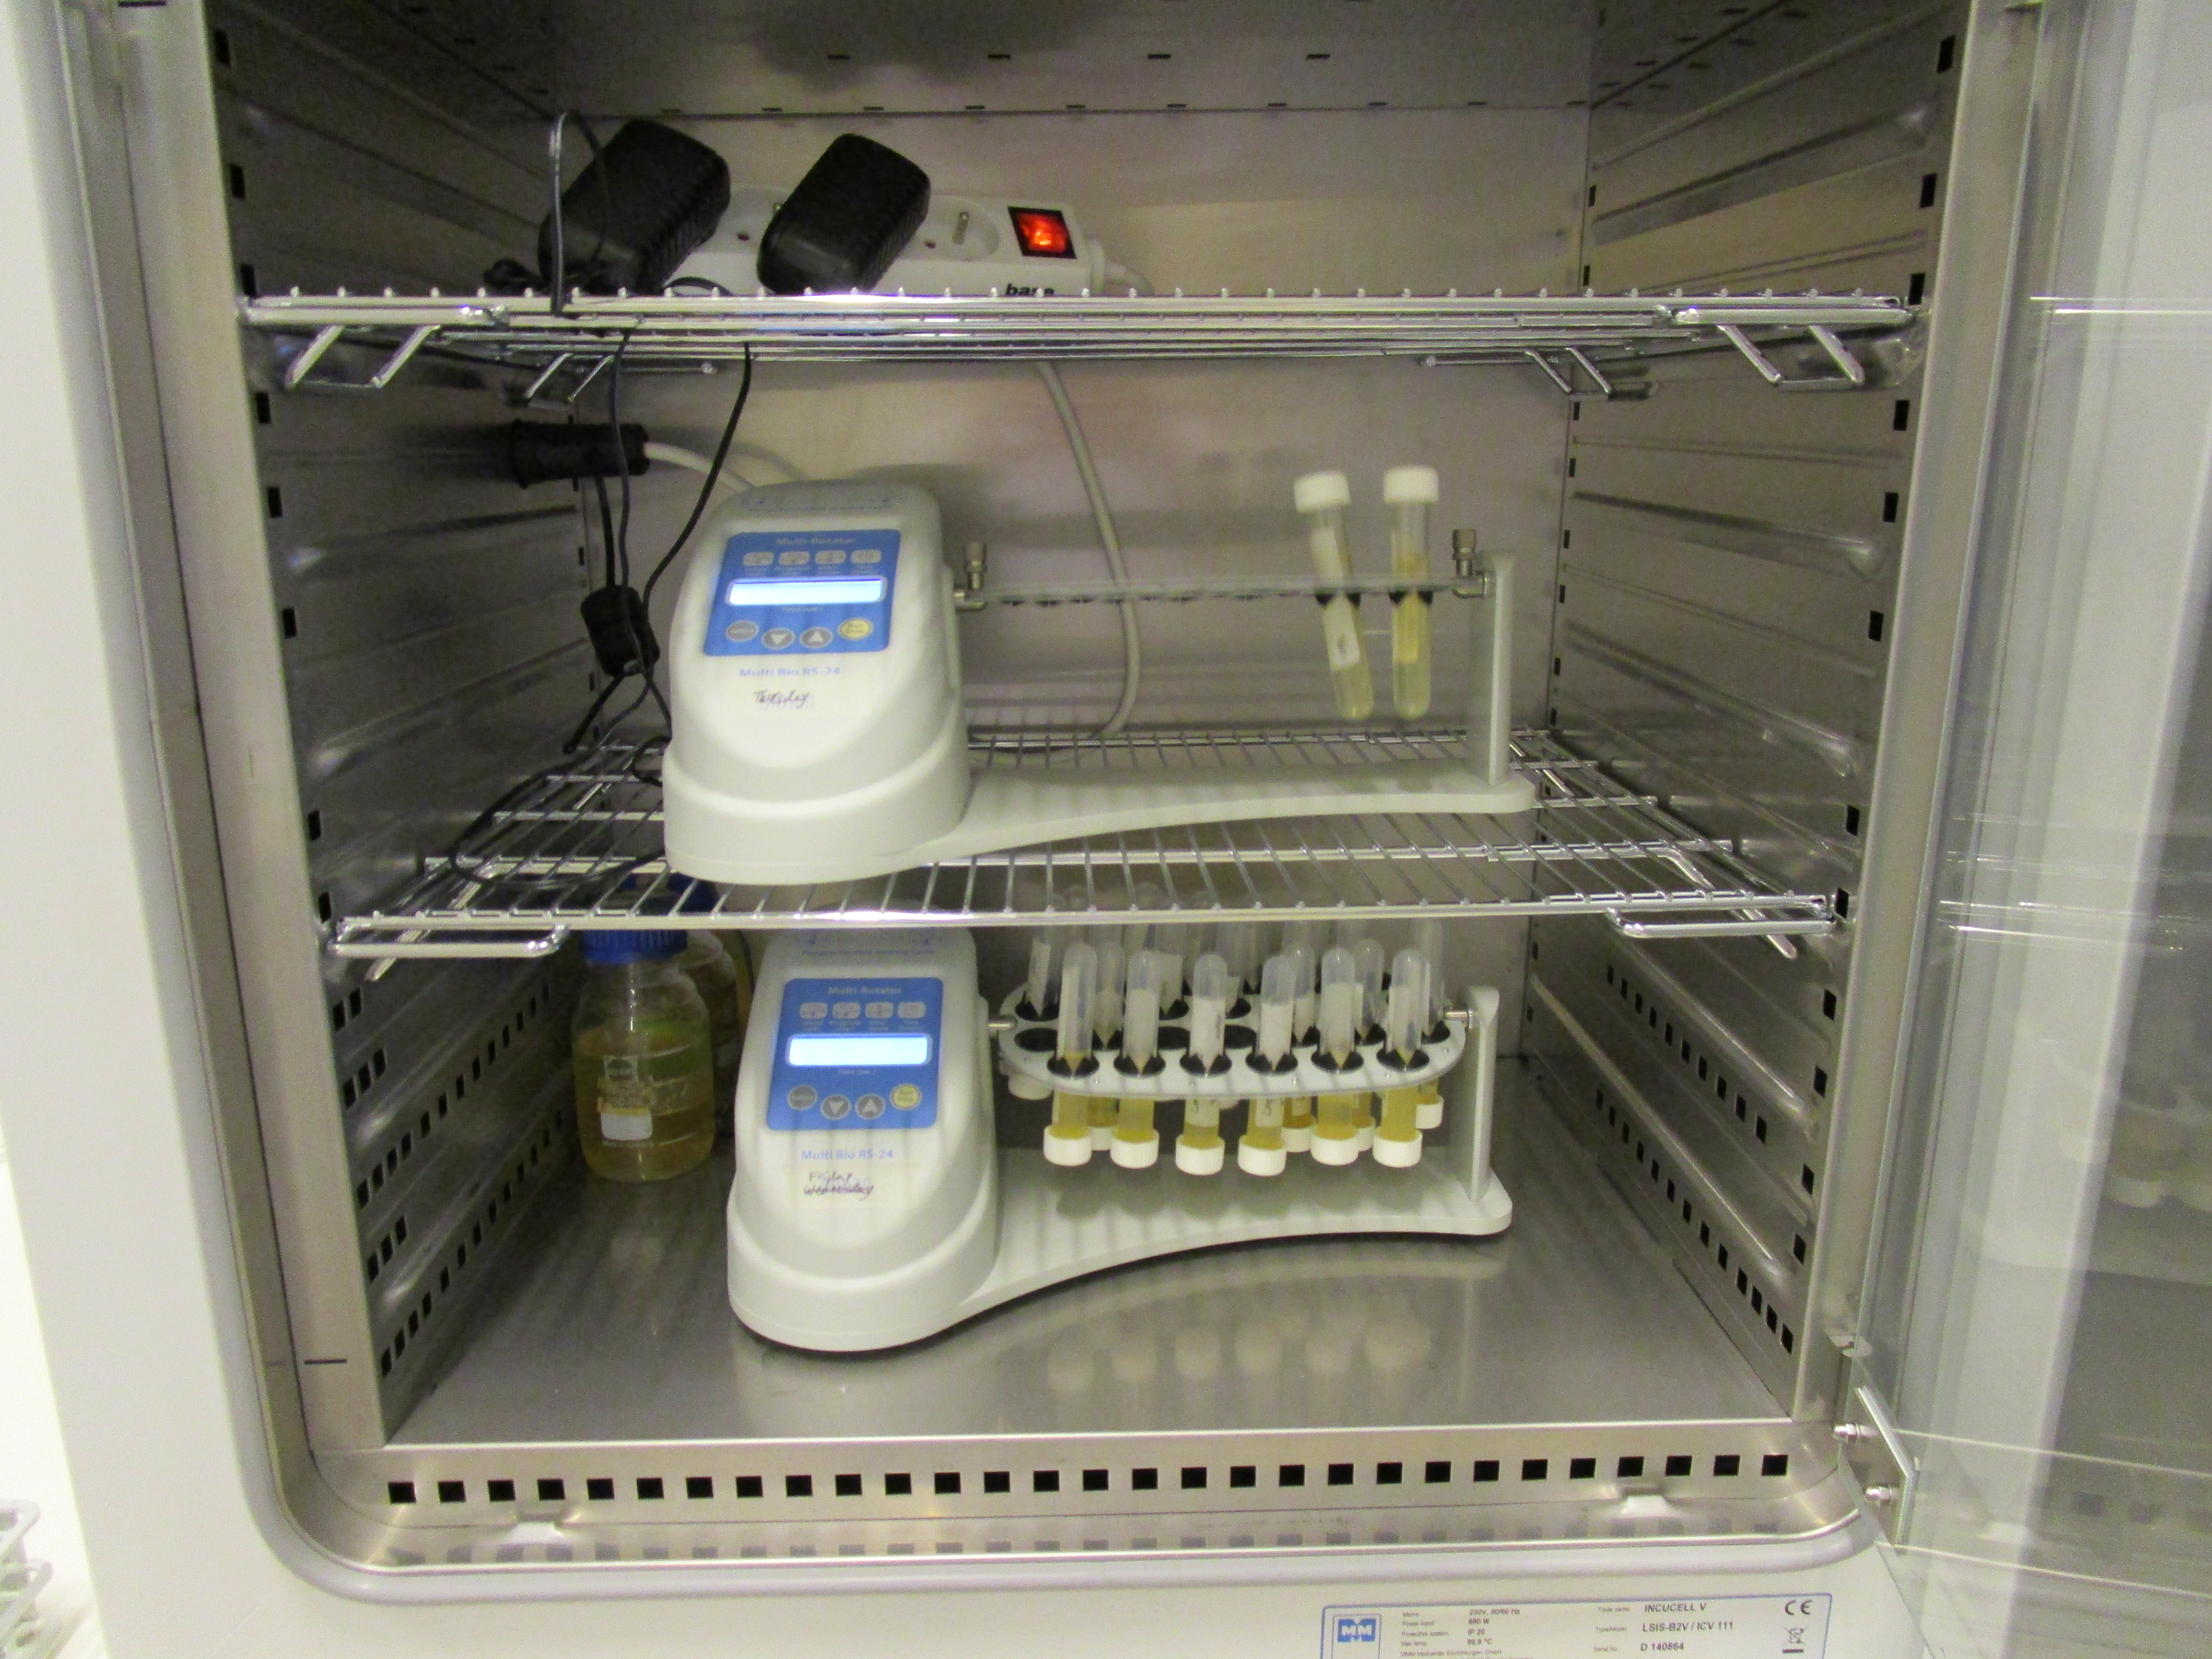
\includegraphics[scale = .01, trim = 5 5 5 5, clip]{incubator.jpg} };
    \node[inner sep = 0 pt] (FCdilutions) at(0, 2.25)
    	{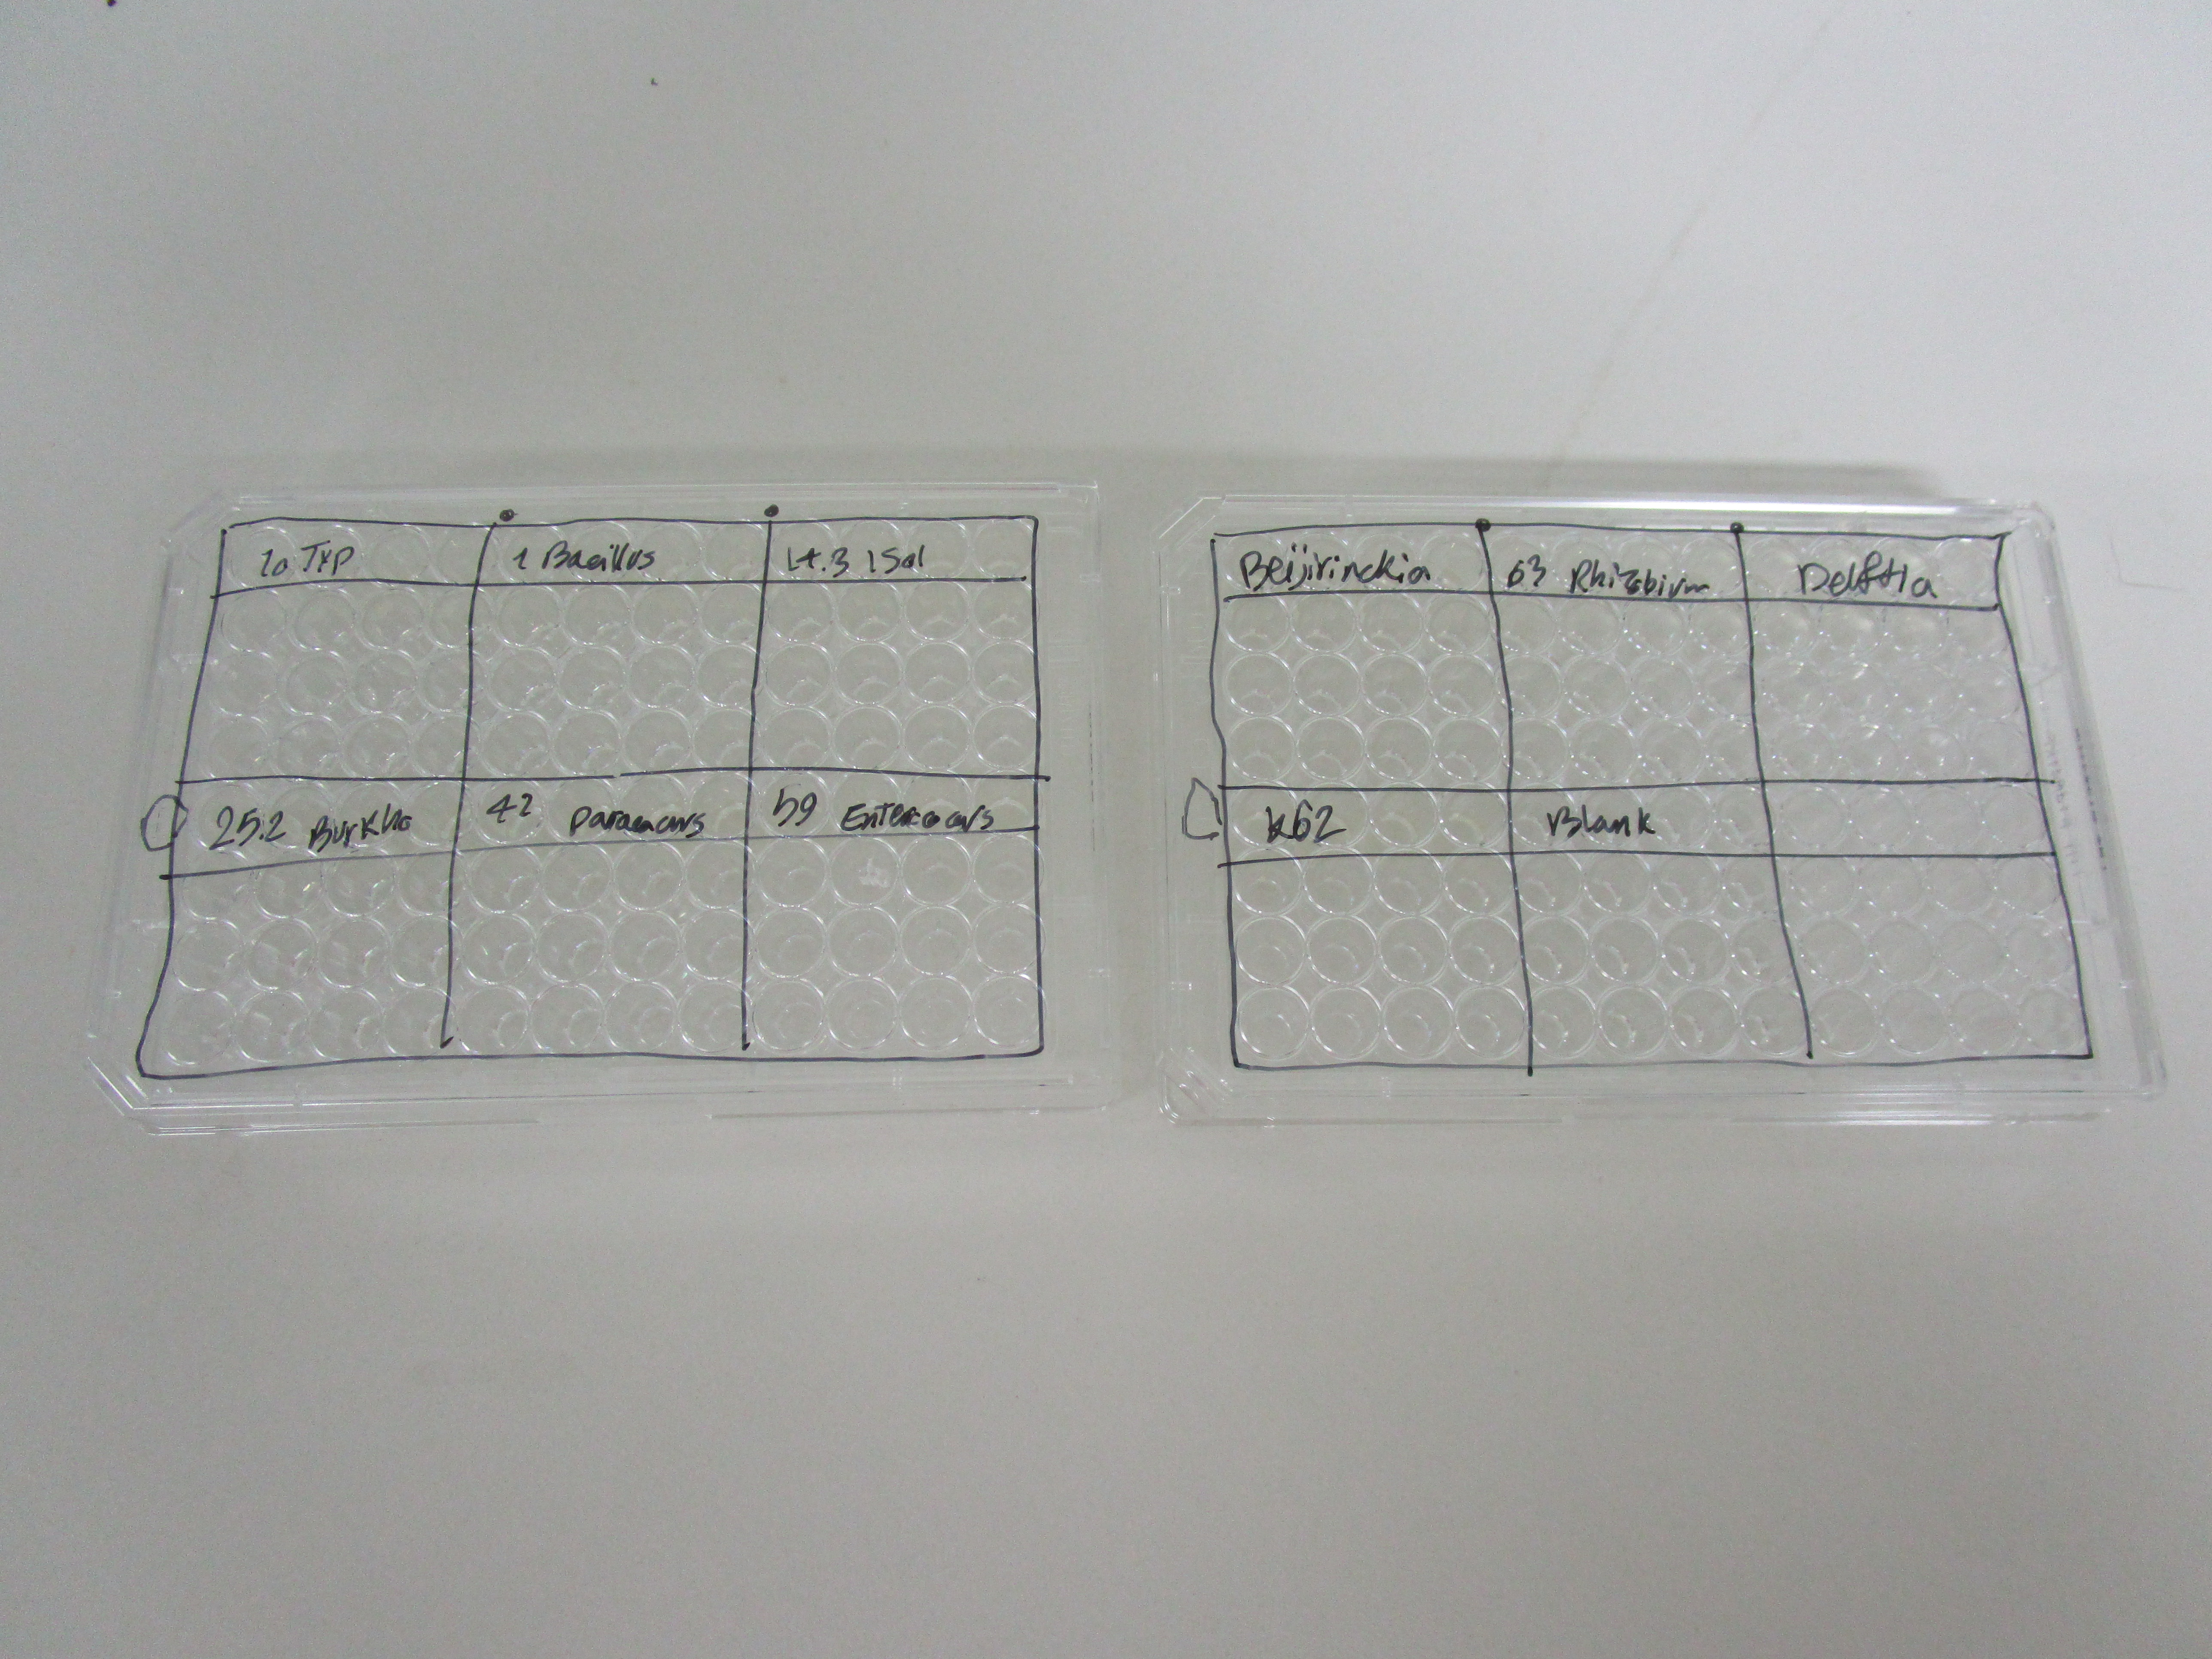
\includegraphics[scale = .01, trim = 5 5 5 5, clip]{FCdilutions.jpg}};
    \node[inner sep = 0 pt] (flowcytometer) at(0, 0)
    	{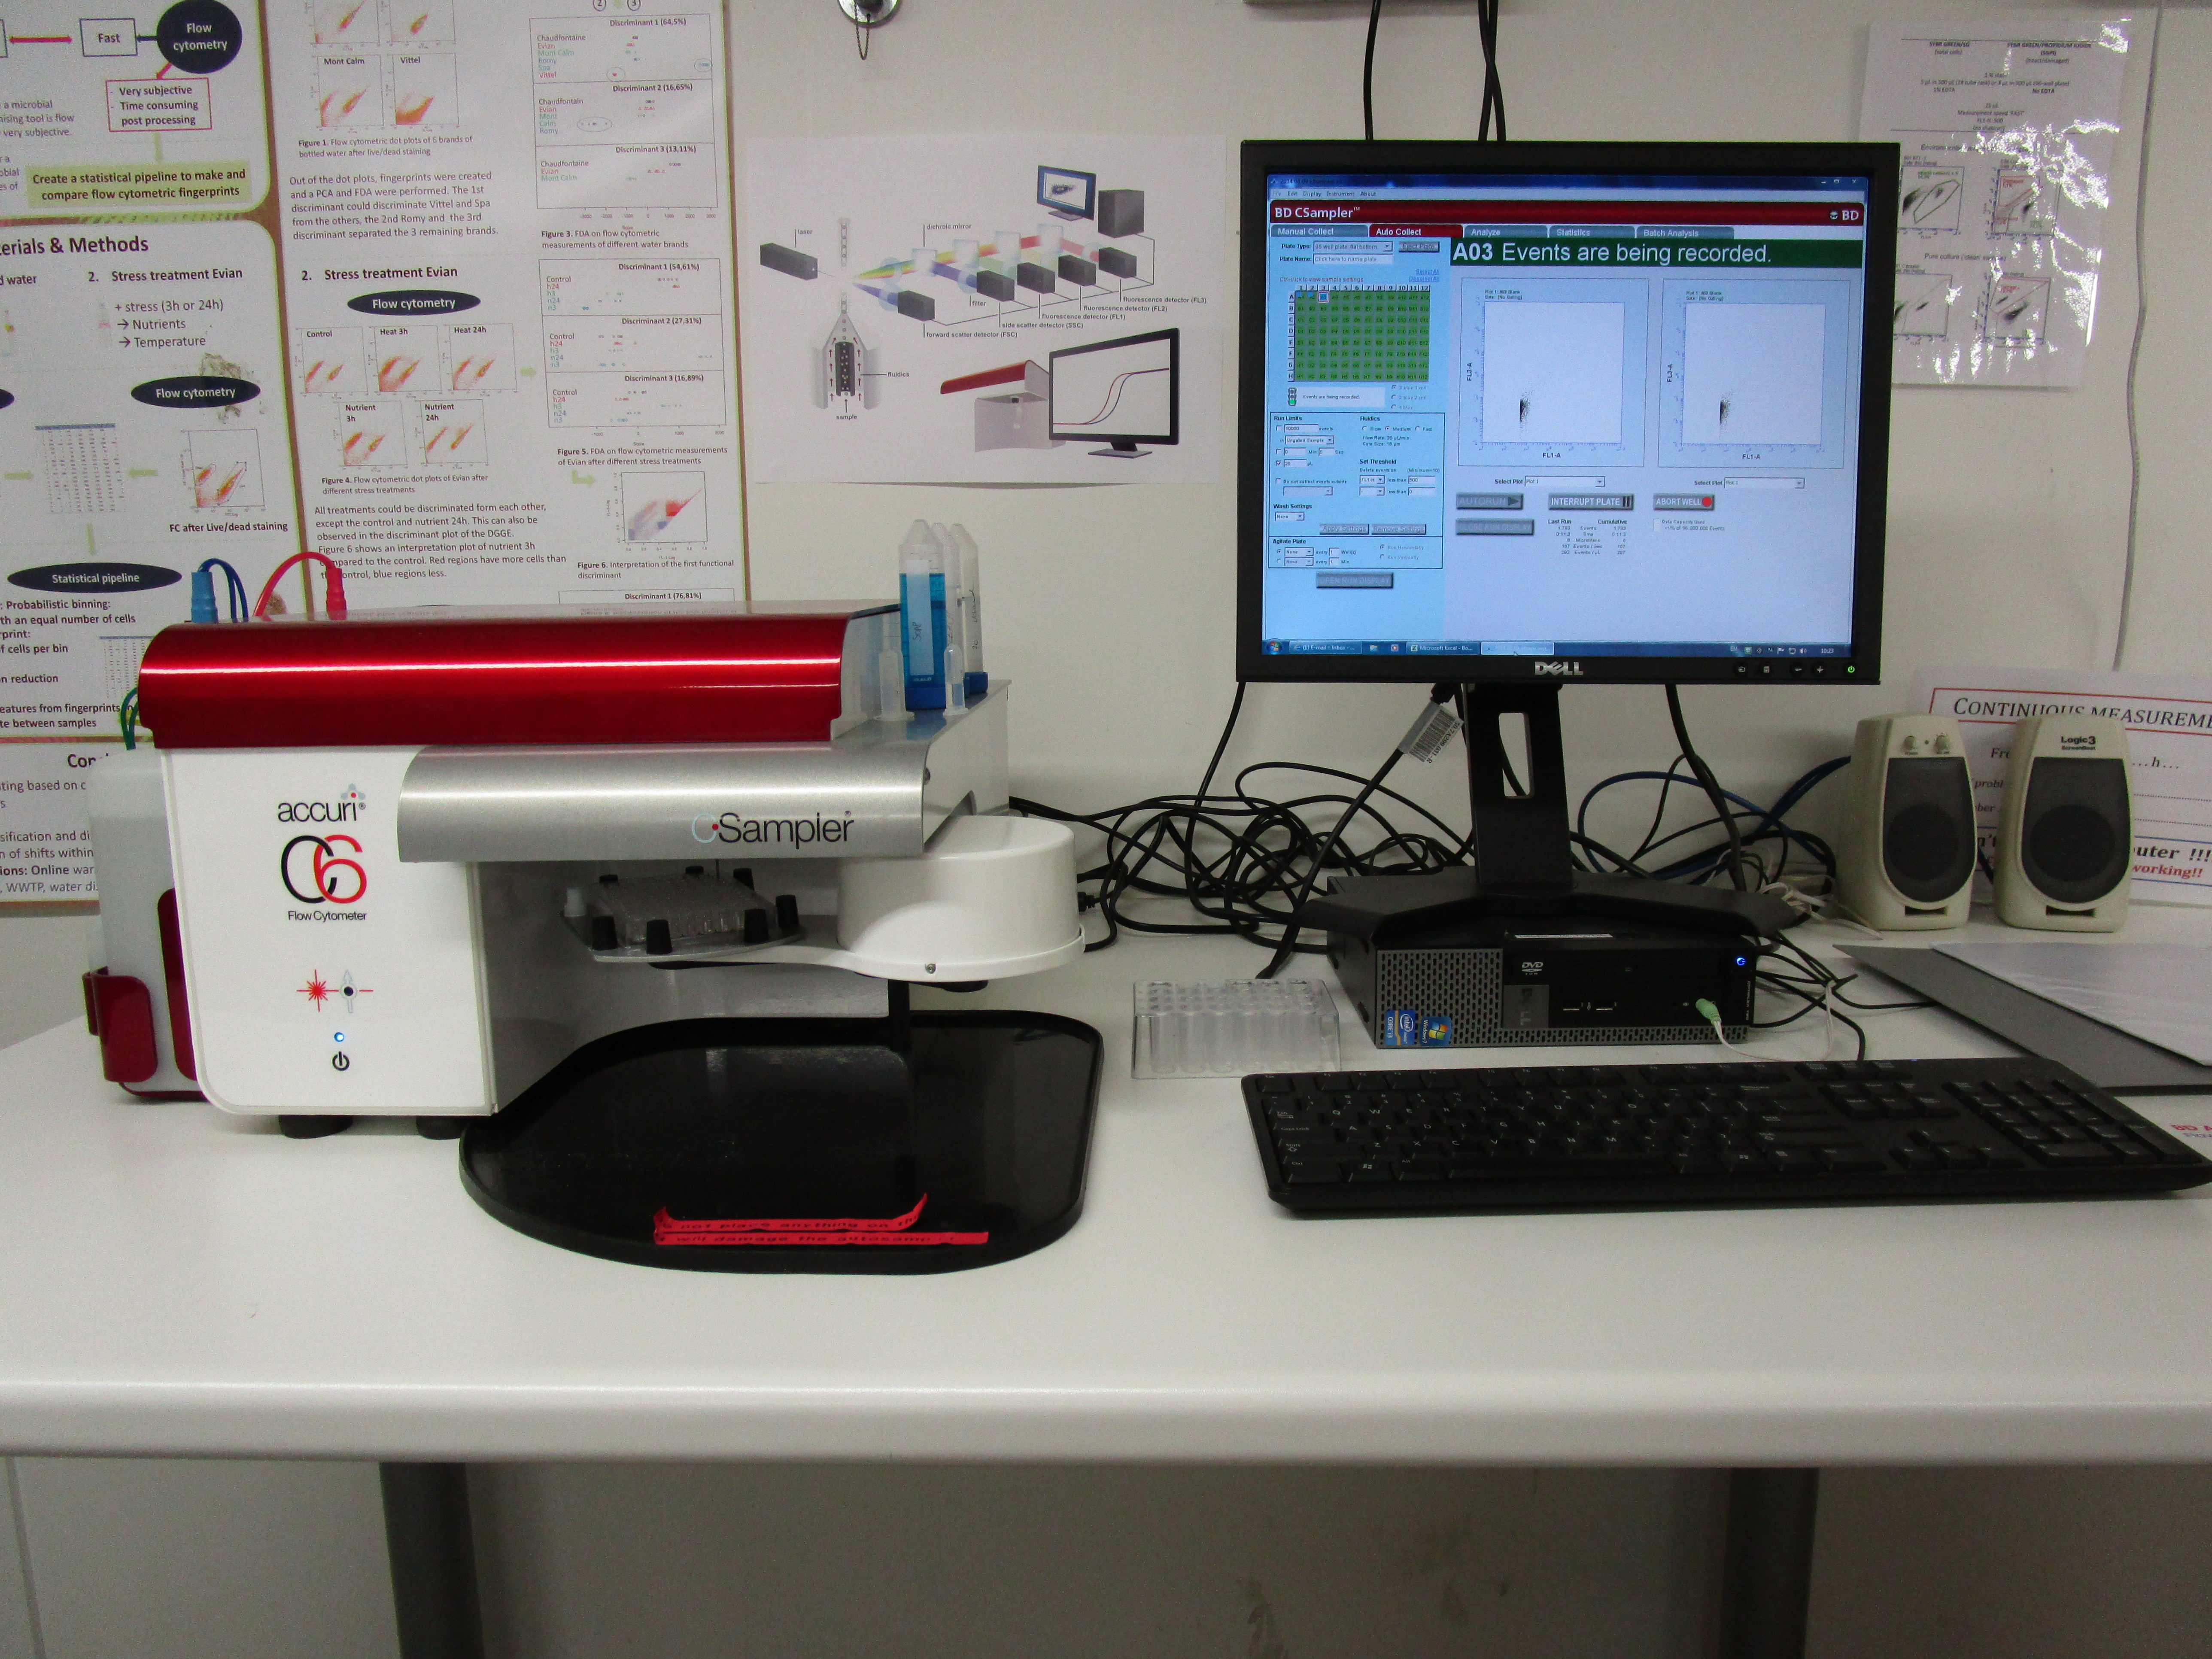
\includegraphics[scale = .01, trim = 5 5 5 5, clip]{flowcytometer.jpg}};
    \node[inner sep = 0 pt] (sampledilutions) at(6, 4.5)
       	{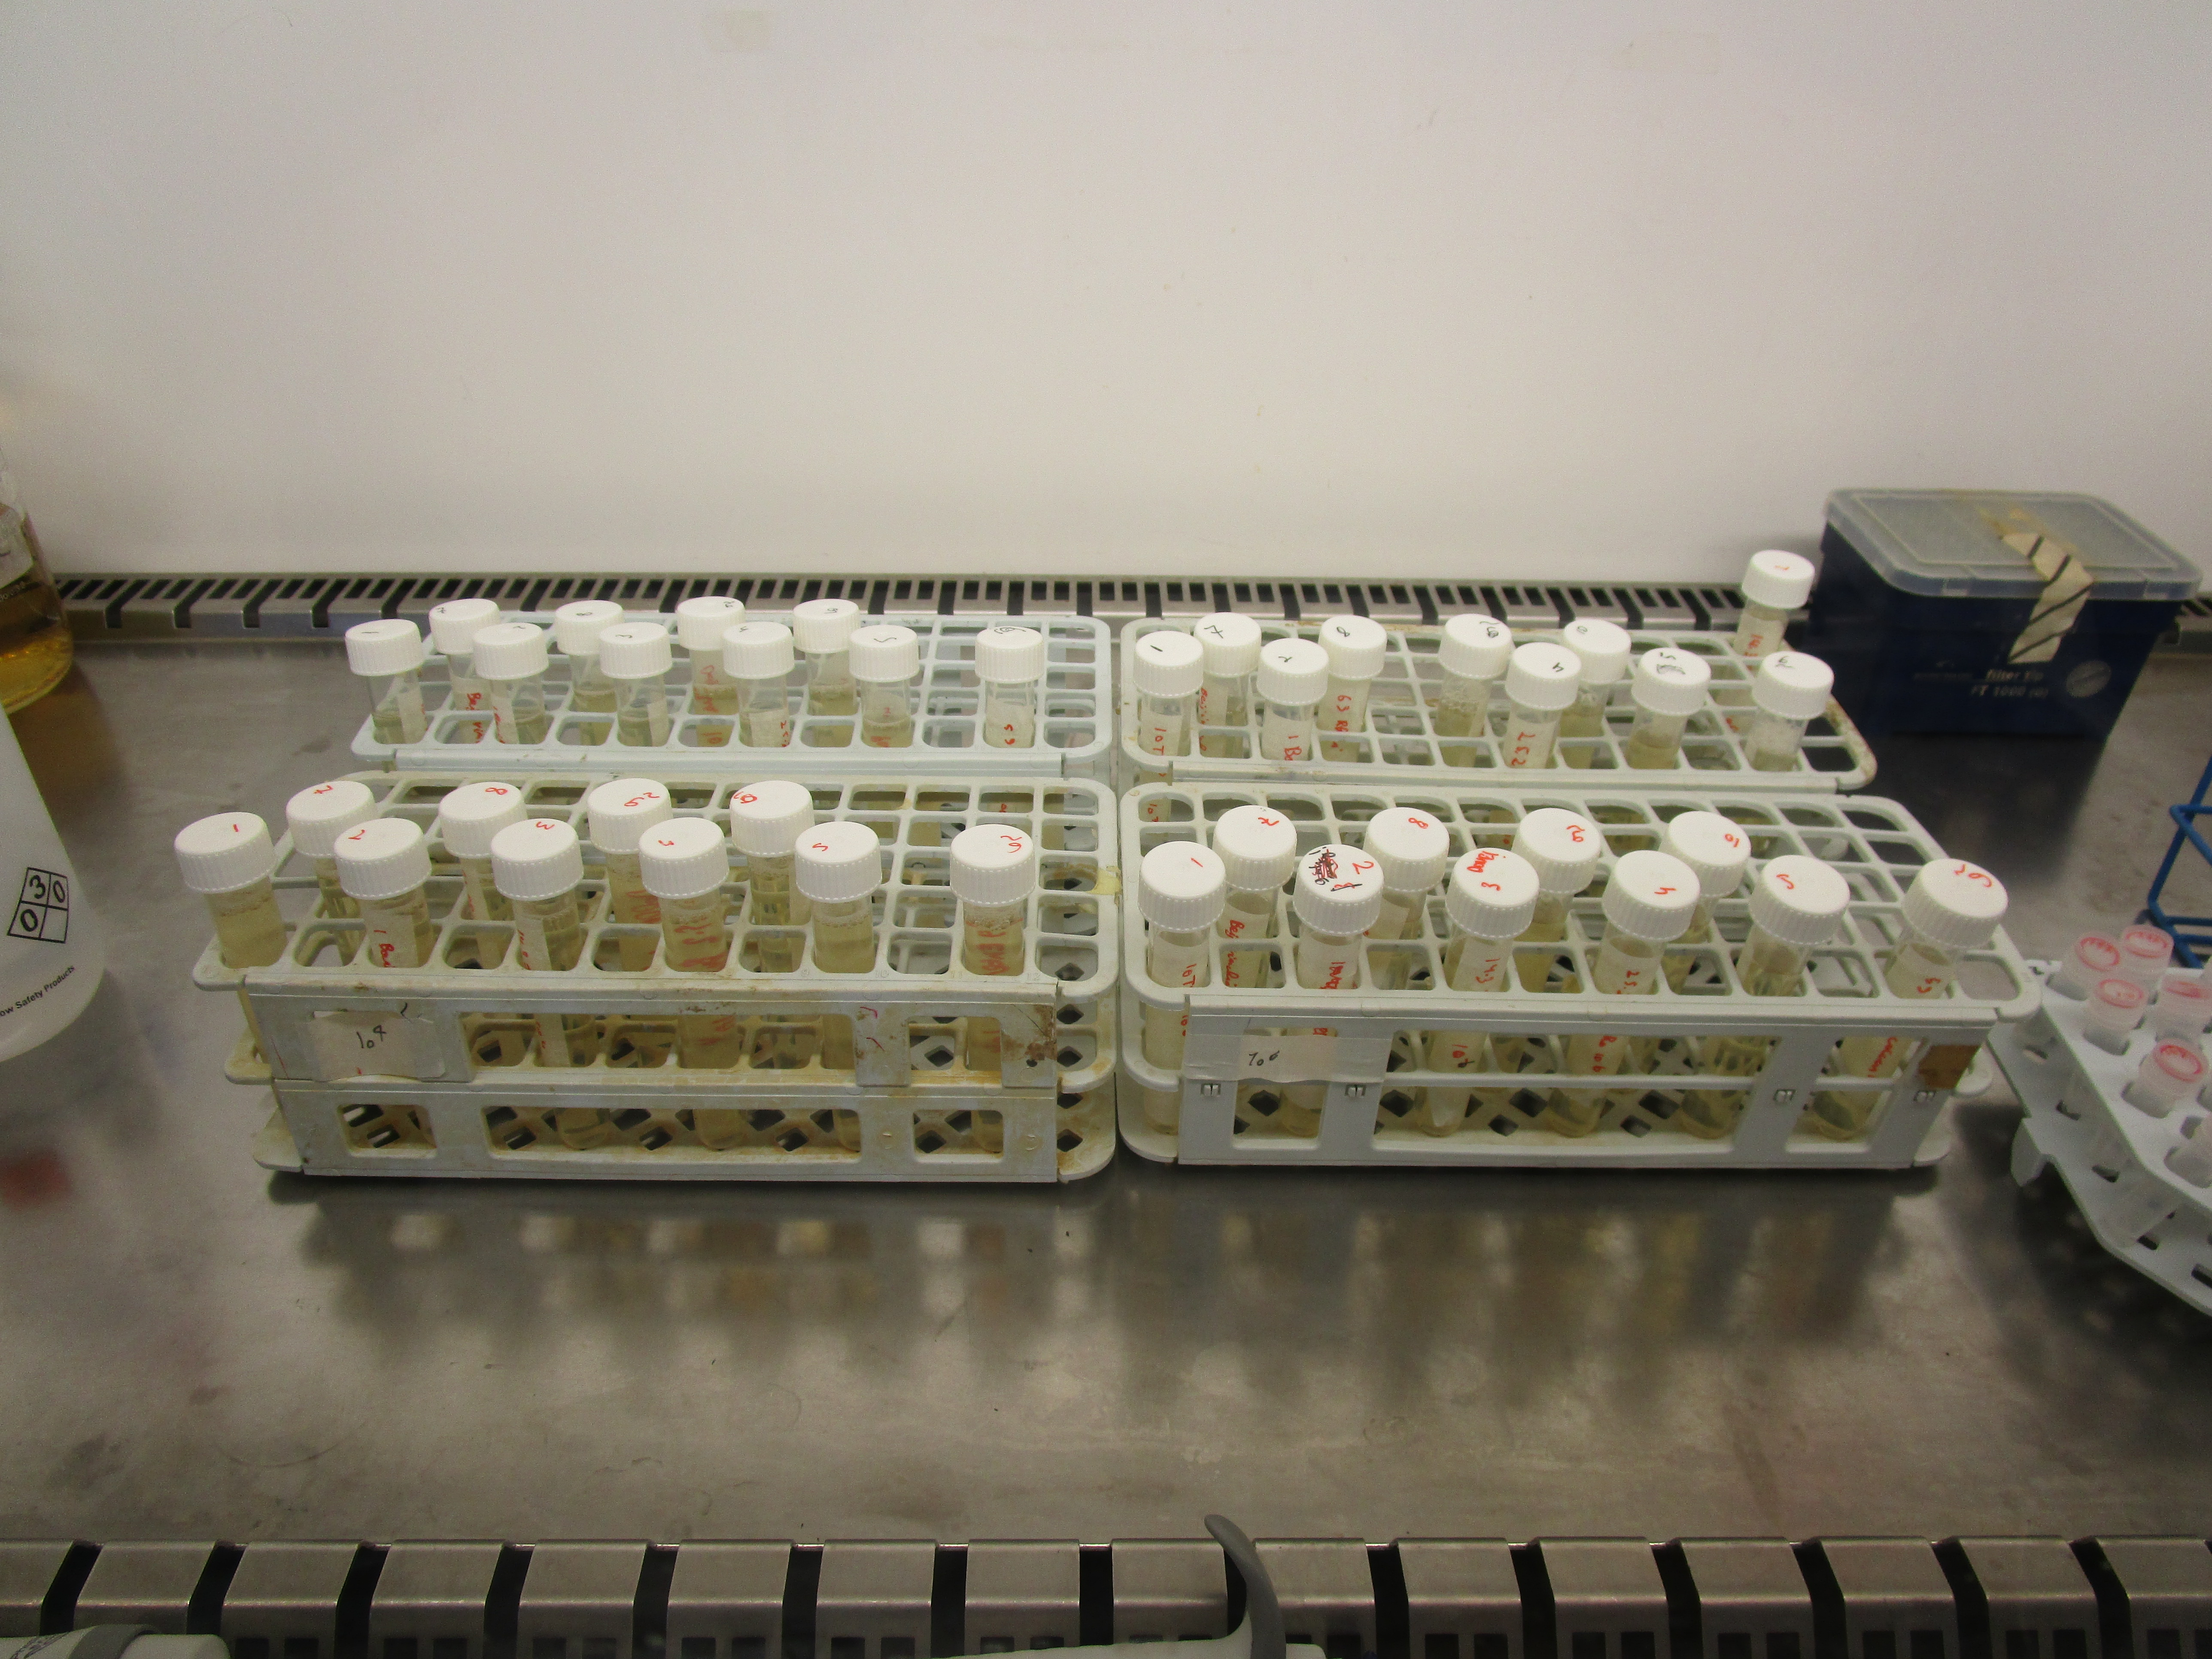
\includegraphics[scale = .01, trim = 5 5 5 5, clip]{sampledilutions.jpg}};
    \node[inner sep = 0 pt] (cryovials) at(6, 2.25)
       	{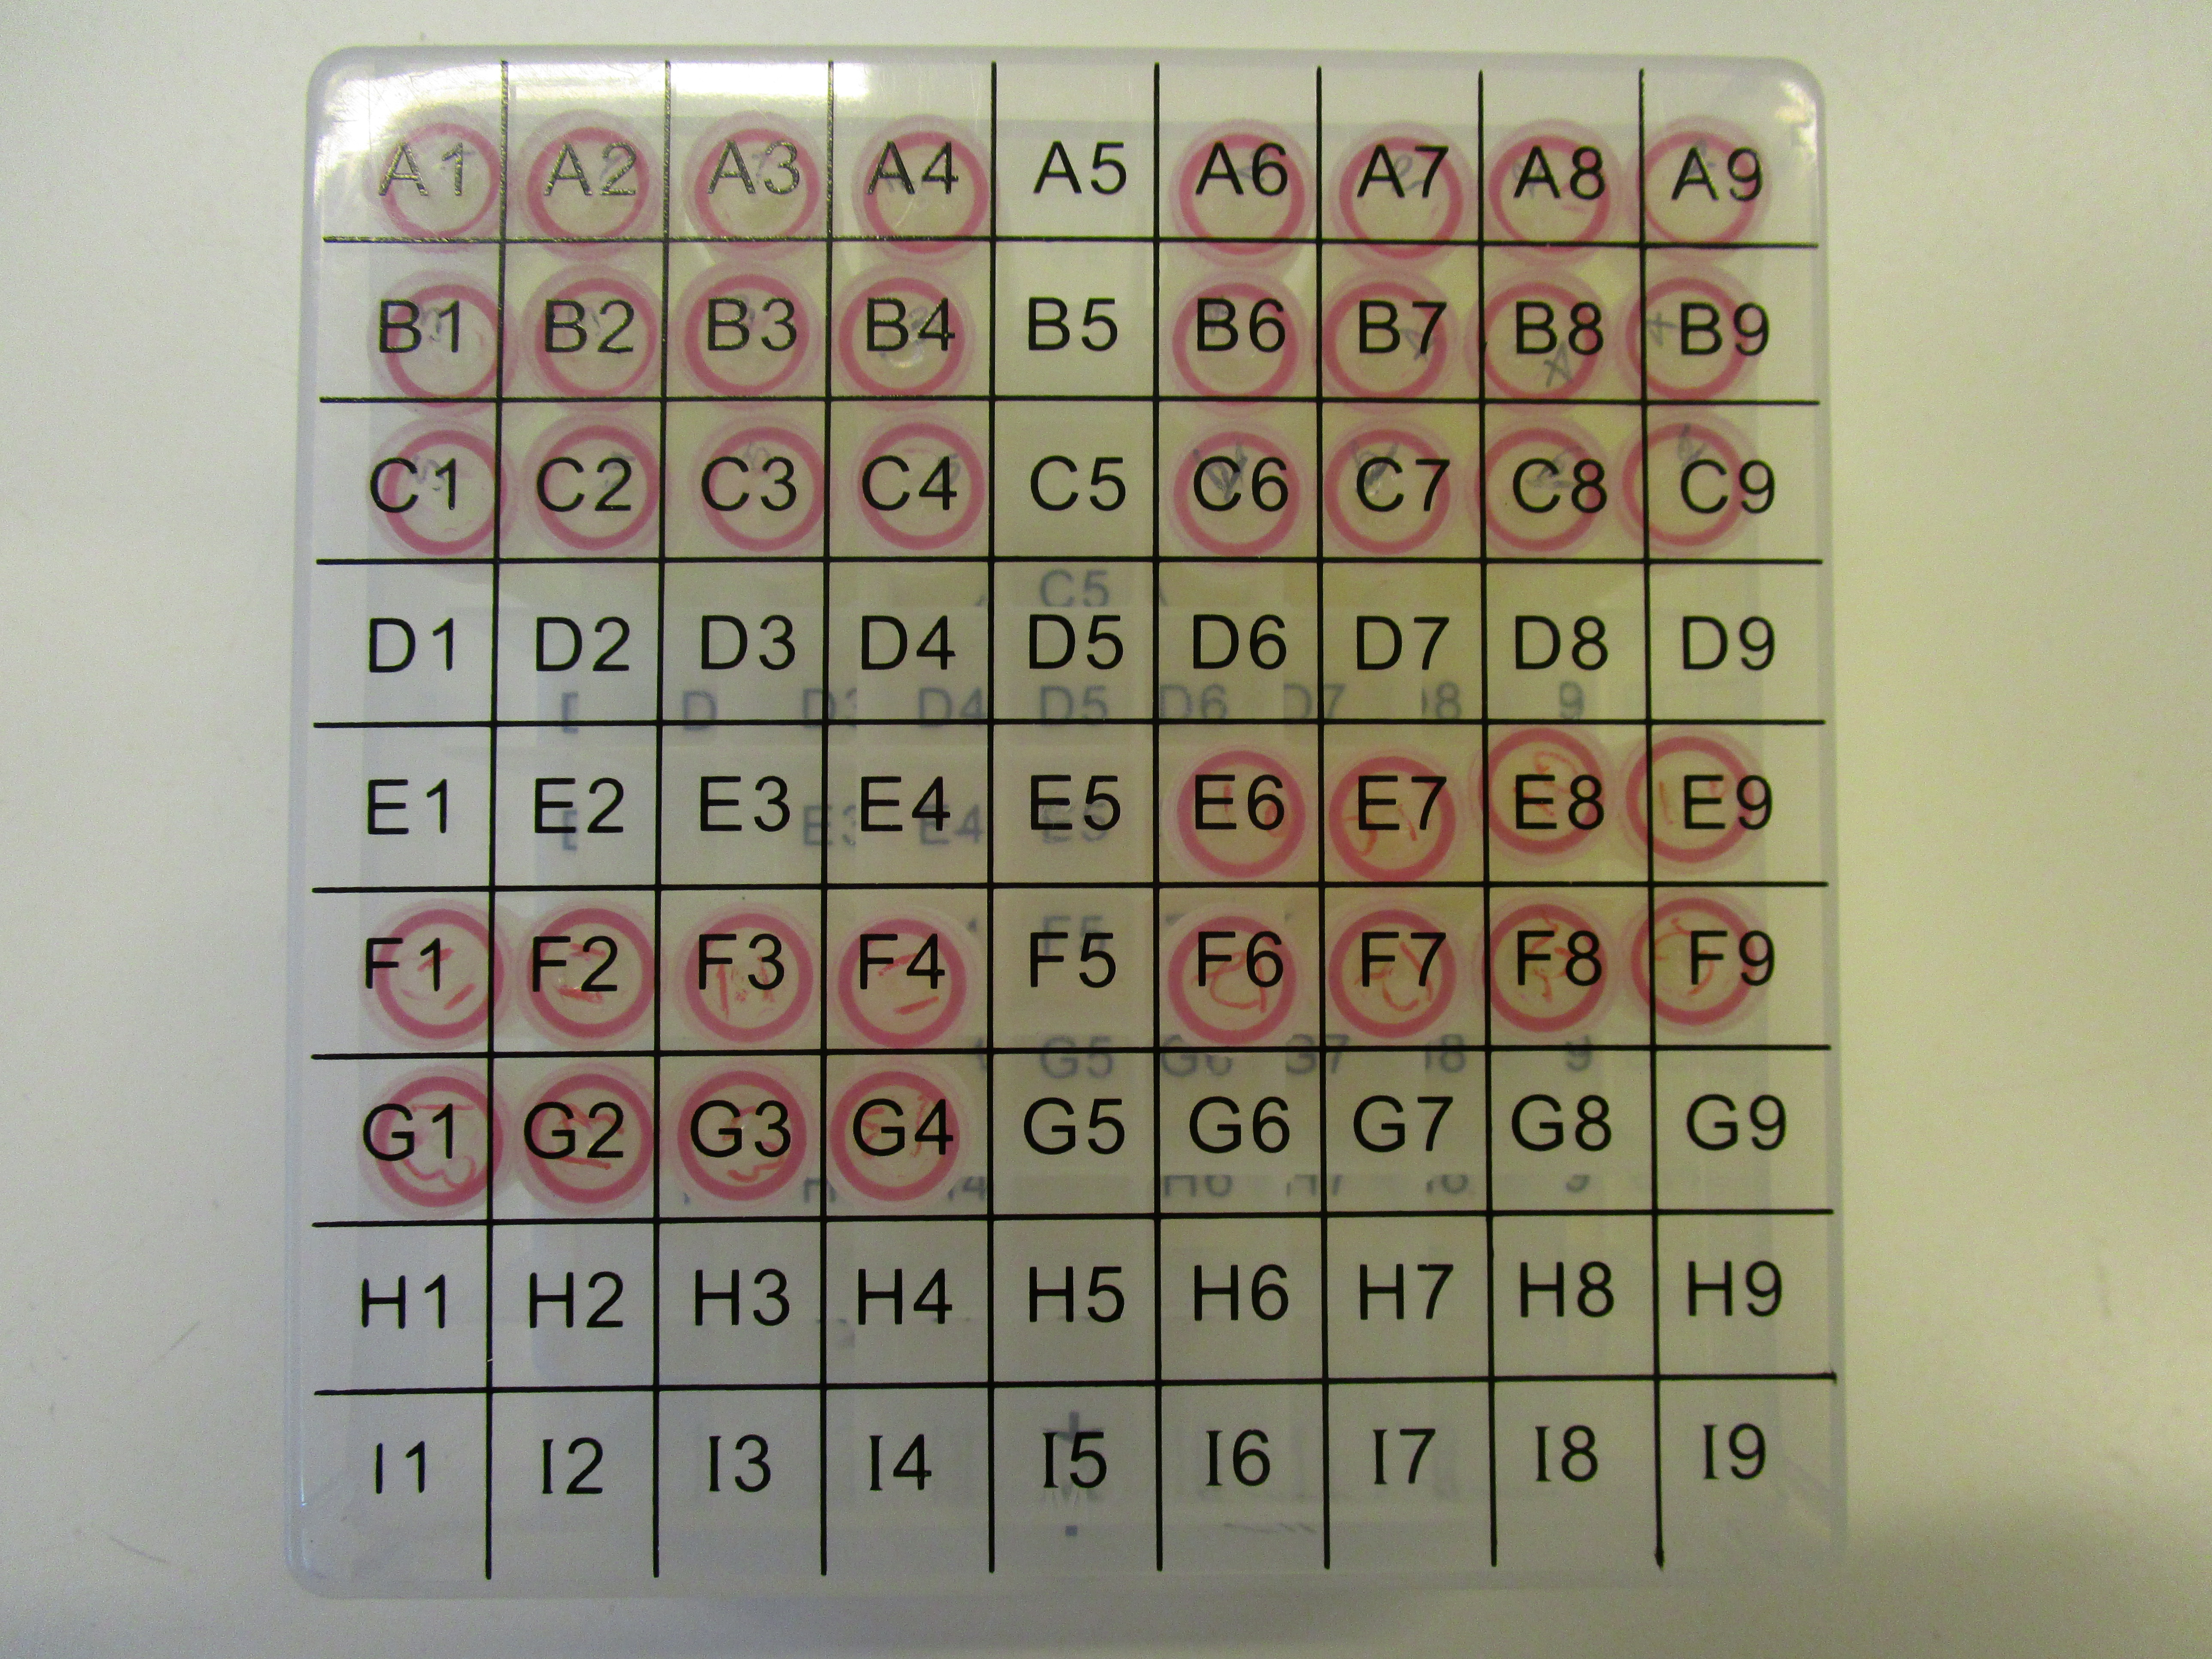
\includegraphics[scale = .01, trim = 5 5 5 5, clip]{cryovials.jpg}};
    \node (freezer) at (6, .5){freeze at -80\degree C};       	
    % Draw some arrows
    %\draw[->] (0,0) -- (7,0) node[center] {FCdilutions};
	\draw[->,thick] (incubator.south) -- (FCdilutions.north)
    	node[midway,fill=white] {preparing dilutions};    
	\draw[->,thick] (FCdilutions.south) -- (flowcytometer.north)
    	node[midway,fill=white] {quantifying cell count};    	
    \draw [thick, ->](flowcytometer) .. controls ([yshift=-3cm, xshift=4cm] flowcytometer) and ([xshift=-3cm] sampledilutions) .. (sampledilutions)
    	node[midway,fill=white] {dilute sample};
	\draw[->,thick] (sampledilutions.south) -- (cryovials.north)
    	node[midway,fill=white] {pipet cultures};     
	\draw[->,thick] (sampledilutions.south) -- (cryovials.north)
    	node[midway,fill=white] {pipet cultures}; 	
	\draw[->,thick] (cryovials.south) -- (freezer.north);  	
	% Draw some accolades
    \draw [decorate,decoration={brace,amplitude=10pt,raise=4pt},yshift=0pt]
    (-1.5,-1) -- (-1.5,5.2) node [black,midway,xshift=-1.2cm] {8-13h};
    \draw [decorate,decoration={brace,amplitude=10pt, mirror,raise=4pt},yshift=0pt]
    (7.3,3.8) -- (7.3,5.2) node [black,midway,xshift=1.2cm] {13-14h};    
    \draw [decorate,decoration={brace,amplitude=10pt, mirror,raise=4pt},yshift=0pt]
    (7.3,0.2) -- (7.3,3) node [black,midway,xshift=1.2cm] {14-18h};        
\end{tikzpicture}
}
\end{frame}

\begin{frame}
\frametitle{Selecting pathogen}
\textbf{Reviving pathogen}
\begin{itemize}
\item Pathogen from one phylogenetic family are chosen.
\item Cultured in nutrient broth and LB broth.
\end{itemize}
\textbf{Making them resistant to antibiotics}
\begin{itemize}
\item Subject them to a concentration gradient of Streptomycin.
\item Subject them to a concentration gradient of Spectinomycin.
\end{itemize}
\end{frame}

\begin{frame}
\frametitle{Results obtained}
\setbeamercolor{block title}{use=structure,fg=white,bg=blue!75!black}
\setbeamercolor{block body}{use=structure,fg=black,bg=white!20!white}

\textbf{Overall progress}\\
\begin{tabular}{l c c}
\hline
Task & Progress \\
\hline
Freeze all 194 communities & \checkmark \\
Make pathogen streptomycin resistant & $\pm$ \\
Pathogen frozen & 2 \\
Invade community and count colonies & 1 pathogen\\
\hline
\end{tabular}
\medskip

\textbf{Statistics}
\begin{block}{Definition model: Poisson Regression}
$$
\log{(\lambda)} = \beta_0 + \beta_1 \times \log(cellcount) + \beta_2 \times evenness + \epsilon
$$
\end{block}
\begin{alltt}\footnotesize
\begin{tabular}{l c c c}
\hline
Coefficients & estimate & Pr(>|z|) & significance\\
\hline
(Intercept) & 5.19089 &  <2e-16 & \text{***} \\
evenness & -0.83349 & <2e-16 & \text{***} \\
log(cellcount) & -0.20031 & <2e-16 & \text{***} \\
\hline
\end{tabular}
\end{alltt}

\footnotesize
No interaction between evenness and $\log{(cellcount)}$: (p-value = 0.185)
\medskip
\end{frame}

\begin{frame}
\frametitle{Future work}
\textbf{End of January}\\
Invade communities with 3 to 6 pathogen \\
\medskip

\textbf{Next semester}\\
Apply predictive modeling to dataset\\
\medskip
\textbf{Possible objectives}
\begin{itemize}
\item Modeling the pathogen growth after 48h.
\item Clustering the communities that are most resilient to pathogen invasion.
\end{itemize}
\end{frame}

\begin{frame}
\frametitle{What's in my dataset?}
\textbf{Variables}
\begin{itemize}
\item id
\item cell count of each bacteria
\item evenness, gini-coefficient and other diversity indices
\item phylogenetic data
\item replica
\item pathogen count
\end{itemize}
\end{frame}

%\begin{frame}
%\frametitle{Acknowledgements}
%\begin{itemize}
%\item Prof. Dr. Peter Vandamme
%\item Dr. Kim Heylen
%\item Dr. Massimo Marzorati 
%\item Elham Ehsani
%\item Tim Lacoere 
%\item Jana De Bodt 
%\item Ir. Benjamin Buysschaert 
%\item people from the EPIC-cluster
%\end{itemize}
%\end{frame}

%------------------------------------------------
%\section{Probleembeschrijving}
%%------------------------------------------------
%
%\begin{frame}
%\frametitle{Probleembeschrijving}
%\textbf{Verspreiding van epidemie}
%\begin{itemize}
%
%\item Geografische verspreiding van epidemische ziekte is niet zo goed begrepen
%\item Temporele ontwikkeling en controle van ziekte zijn beter begrepen
%\item Diffusiemodel voor de verspreiding van algemene epidemie kan inzicht brengen
%
%
%\end{itemize}
%\end{frame}
%%
%%%------------------------------------------------
%
%\begin{frame}
%\frametitle{Defini\"{e}ring vergelijkingen}
%
%Er werd gekozen voor een vereenvoudigd stelsel van vergelijkingen uit \cite{murray2003mathematical}.
%
%\begin{gather}\label{equations1}
%\left\{
%	\begin{array}{ll}
%	\frac{\partial S}{\partial T} = - \beta IS+D_S(\frac{\partial^2S}{\partial X^2}+\frac{\partial^2S}{\partial Y^2})\\
%	\frac{\partial I}{\partial T} = \beta IS -\sigma I +D_I(\frac{\partial^2I}{\partial X^2}+\frac{\partial^2I}{\partial Y^2})\\
%	\frac{\partial R}{\partial T} = \sigma I + D_R(\frac{\partial^2R}{\partial X^2}+\frac{\partial^2R}{\partial Y^2}) 
%	\end{array}
%\right.	
%\end{gather}
%
%\begin{itemize}
%\item $S[km^{-2}], I[km^{-2}]$ en $R[km^{-2}]$ stellen de proportionele densiteit voor van resp. ``susceptible", ``infected'' en ``recovered" 
%\item $\beta$ [km$^2$ jaar$^{-1}$] staat voor de ziekteoverdracht
%\item $1/\sigma$ [jaar] is de incubatietijd van de ziekte
%\item $D_S, D_I$ en $D_R$ zijn de diffusieco\"{e}ffici\"{e}nten.
%\end{itemize}
%
%\end{frame}
%
%\begin{frame}
%\frametitle{Opmerking vereenvoudiging}
%\begin{itemize}
%\item Door vereenvoudiging van vgl.-en wordt N constant, i.e. $N = S+I+R$.
%\item De initieel gekozen N varieert niet.
%\end{itemize}
%\begin{align*}
%\frac{\partial N}{\partial T} &= \frac{\partial S}{\partial T} + \frac{\partial I}{\partial T} + \frac{\partial R}{\partial T}\\
%&= - \beta RS+D_S\nabla^2 S + \beta RS -\sigma I +D_I\nabla^2 
%I + \sigma I + D_R\nabla^2 R\\
%&=D_S\nabla^2 S + D_I\nabla^2 I + D_R\nabla^2 R,
%\end{align*}
%\end{frame}
%
%
%\begin{frame}
%\frametitle{Parameterbeschrijving}
%\begin{table}[h]
%\centering
%\begin{tabular}{l c c}
%\hline
%Parameter & Symbol & Value \\
%\hline
%Average incubation time & $\frac{1}{\sigma}$ & 28 / 365 year\\
%Disease transmission coefficient & $\beta$ & 15 km$^2$ year$^{-1}$\\
%Diffusion coefficient of the susceptibles & $D_S$ & 0.05 km$^2$ year$^{-1}$\\
%Diffusion coefficient of the infected & $D_I$ & 0.02 km$^2$ year$^{-1}$\\
%Diffusion coefficient of the recovered & $D_R$ & 0.01 km$^2$ year$^{-1}$\\
%\hline
%\end{tabular}
%\caption{Parameter description}
%\label{tabel1}
%\end{table}
%\end{frame}
%
%\section{Domeinafbakening}
%
%\begin{frame}
%\frametitle{Domeinafbakening}
%Het domein wordt afgebakend als $(x,y,t) \in [0,20] \times [0,20] \times [0,50]$ waarbij initi\"{e}le en boundary conditions:
%
%\begingroup
%    \fontsize{7pt}{12pt}\selectfont
%  \begin{multicols}{3}
%  
%  \begin{gather}\label{boundary1}
%  \left\{
%      \begin{array}{ll}
%      S(x,y,0)&= 1 -I(x,y,0)\\
%      \frac{\partial S(0,y,t)}{\partial x}&= 0, t > 0\\
%      \frac{\partial S(x,0,t)}{\partial y})&=0, t > 0\\
%      \frac{\partial S(20,y,t)}{\partial x}&= 0, t > 0\\
%      \frac{\partial S(x,20,t)}{\partial y}&= 0, t > 0\\
%      \end{array}
%  \right.
%  \end{gather}
%  
%  \begin{gather}\label{boundary2}
%  \left\{
%      \begin{array}{ll}
%      I(x,y,0)&= e^{(-(x-10)^2-(y-10)^2)}\\
%      \frac{\partial I(0,y,t)}{\partial x}&= 0, t > 0\\
%      \frac{\partial I(x,0,t)}{\partial y})&=0, t > 0\\
%      \frac{\partial I(20,y,t)}{\partial x}&= 0, t > 0\\
%      \frac{\partial I(x,20,t)}{\partial y}&= 0, t > 0\\
%      \end{array}
%  \right.
%  \end{gather}
%  
%  \begin{gather}\label{boundary3}
%  \left\{
%      \begin{array}{ll}
%      R(x,y,0)&= 0\\
%      \frac{\partial R(0,y,t)}{\partial x}&= 0, t > 0\\
%      \frac{\partial R(x,0,t)}{\partial y})&=0, t > 0\\
%      \frac{\partial R(20,y,t)}{\partial x}&= 0, t > 0\\
%      \frac{\partial R(x,20,t)}{\partial y}&= 0, t > 0\\
%      \end{array}
%  \right.
%  \end{gather}    
%  \end{multicols}
%\endgroup
%
%\end{frame}
%
%\section{Schema uitwerking}
%
%\begin{frame}
%\frametitle{Uitwerking schema}
%Vergelijkingen (\ref{equations1}) kunnen uitgewerkt worden volgens een expliciet schema.
%
%\begin{gather*}\label{equations2}
%\left\{
%	\begin{array}{ll}
%	\frac{S_{i,j}^{k+1}-S_{i,j}^{k}}{\Delta t} = - \beta R^k_{i,j}S^k_{i,j}+D_S\big(\frac{S_{i+1,j}^{k}-2S_{i,j}^{k}+S_{i-1,j}^{k}}{\Delta x^2}+\frac{S_{i,j+1}^{k}-2S_{i,j}^{k}+S_{i,j-1}^{k}}{\Delta y^2}\big)\\
%	\frac{I_{i,j}^{k+1}-I_{i,j}^{k}}{\Delta t} = \beta R^k_{i,j}S^k_{i,j} -\sigma I^k_{i,j} +D_I\big(\frac{I_{i+1,j}^{k}-2I_{i,j}^{k}+I_{i-1,j}^{k}}{\Delta x^2}+\frac{I_{i,j+1}^{k}-2I_{i,j}^{k}+I_{i,j-1}^{k}}{\Delta y^2}\big)\\
%	\frac{R_{i,j}^{k+1}-R_{i,j}^{k}}{\Delta t} = \sigma I^k_{i,j} + D_R\big(\frac{R_{i+1,j}^{k}-2R_{i,j}^{k}+R_{i-1,j}^{k}}{\Delta x^2}+\frac{R_{i,j+1}^{k}-2R_{i,j}^{k}+R_{i,j-1}^{k}}{\Delta y^2}\big)\\
%	\end{array}
%\right.	
%\end{gather*}
%
%\begin{itemize}
%\item tijdstap $\Delta t = 0.005$ jaar en $\Delta x = \Delta y = 0.5$ km.
%\item welke voldoet aan $\frac{\Delta t}{\Delta x^2} \leq \frac{1}{2}$, nodige voorwaarde voor een convergerende oplossing.
%\end{itemize} 
%\end{frame}
%
%\begin{frame}
%\frametitle{Uitwerking schema}
%Na herschikking worden de vergelijkingen geschreven als:
%\begin{gather*}\label{equations3}
%\left\{
%	\begin{array}{ll}
%	S_{i,j}^{k+1} = \Big[- \beta R^k_{i,j}S^k_{i,j}+D_S\big(\frac{S_{i+1,j}^{k}-2S_{i,j}^{k}+S_{i-1,j}^{k}}{\Delta x^2}+\frac{S_{i,j+1}^{k}-2S_{i,j}^{k}+S_{i,j-1}^{k}}{\Delta y^2}\big)\Big]\Delta t +S_{i,j}^{k}\\
%	I_{i,j}^{k+1} =\Big[ \beta R^k_{i,j}S^k_{i,j} -\sigma I^k_{i,j} +D_I\big(\frac{I_{i+1,j}^{k}-2I_{i,j}^{k}+I_{i-1,j}^{k}}{\Delta x^2}+\frac{I_{i,j+1}^{k}-2I_{i,j}^{k}+I_{i,j-1}^{k}}{\Delta y^2}\big)\Big]\Delta t + I_{i,j}^{k}\\
%	R_{i,j}^{k+1} = \Big[\sigma I^k_{i,j} + D_R\big(\frac{R_{i+1,j}^{k}-2R_{i,j}^{k}+R_{i-1,j}^{k}}{\Delta x^2}+\frac{R_{i,j+1}^{k}-2R_{i,j}^{k}+R_{i,j-1}^{k}}{\Delta y^2}\big)\Big]\Delta t + R_{i,j}^{k}\\
%	\end{array}
%\right.	
%\end{gather*}
%\end{frame}
%
%\begin{frame}
%\frametitle{Uitwerking Schema}
%\textbf{Imaginaire punten}\\
%Om de waarden op de grens van het domein te berekenen worden imaginaire punten gedefinieerd. De Neumann-randvoorwaarden in vgl. (\ref{boundary1}, \ref{boundary2} en \ref{boundary3}) worden gediscretiseerd.
%\begingroup
%    \fontsize{10pt}{12pt}\selectfont
%  \begin{multicols}{3}
%  \begin{gather*}
%  \left\{
%      \begin{array}{ll}
%      \frac{S^{k}_{1,j}-S^{k}_{-1,j}}{2\Delta x}&= 0, t > 0\\
%      \frac{S^{k}_{i,1}-S^{k}_{i,-1}}{2\Delta y}&= 0, t > 0\\
%      \frac{S^{k}_{21,j}-S^{k}_{19,j}}{2\Delta x}&= 0, t > 0\\
%      \frac{S^{k}_{i,21}-S^{k}_{i,19}}{2\Delta y}&= 0, t > 0\\
%      \end{array}
%  \right.
%  \end{gather*}
%  
%  \begin{gather*}
%  \left\{
%      \begin{array}{ll}
%      \frac{I^{k}_{1,j}-I^{k}_{-1,j}}{2\Delta x}&= 0, t > 0\\
%      \frac{I^{k}_{i,1}-I^{k}_{i,-1}}{2\Delta y}&= 0, t > 0\\
%      \frac{I^{k}_{21,j}-I^{k}_{19,j}}{2\Delta x}&= 0, t > 0\\
%      \frac{I^{k}_{i,21}-I^{k}_{i,19}}{2\Delta y}&= 0, t > 0\\
%      \end{array}
%  \right.
%  \end{gather*}
%  
%  \begin{gather*}
%  \left\{
%      \begin{array}{ll}
%      \frac{R^{k}_{1,j}-R^{k}_{-1,j}}{2\Delta x}&= 0, t > 0\\
%      \frac{R^{k}_{i,1}-R^{k}_{i,-1}}{2\Delta y}&= 0, t > 0\\
%      \frac{R^{k}_{21,j}-R^{k}_{19,j}}{2\Delta x}&= 0, t > 0\\
%      \frac{R^{k}_{i,21}-R^{k}_{i,19}}{2\Delta y}&= 0, t > 0\\
%      \end{array}
%  \right.
%  \end{gather*}    
%  \end{multicols}
%\endgroup
%
%\end{frame}
%
%\begin{frame}
%\frametitle{Uitwerking Schema}
%\textbf{Imaginaire punten}\\
%Na herschikking kunnen de zgn. \textit{ghost points} ingevuld worden.
%
%\begingroup
%    \fontsize{10pt}{12pt}\selectfont
%  \begin{multicols}{3}
%  \begin{gather*}
%  \left\{
%      \begin{array}{ll}
%      S^{k}_{-1,j}&= S^{k}_{1,j}, t > 0\\
%      S^{k}_{i,-1}&= S^{k}_{i,1}, t > 0\\
%      S^{k}_{21,j}&= S^{k}_{19,j}, t > 0\\
%      S^{k}_{i,21}&= S^{k}_{i,19}, t > 0\\
%      \end{array}
%  \right.
%  \end{gather*}
%  
%  \begin{gather*}
%  \left\{
%      \begin{array}{ll}
%      I^{k}_{-1,j}&= I^{k}_{1,j}, t > 0\\
%      I^{k}_{i,-1}&= I^{k}_{i,1}, t > 0\\
%      I^{k}_{21,j}&= I^{k}_{19,j}, t > 0\\
%      I^{k}_{i,21}&= I^{k}_{i,19}, t > 0\\
%      \end{array}
%  \right.
%  \end{gather*}
%  
%  \begin{gather*}
%  \left\{
%      \begin{array}{ll}
%      R^{k}_{-1,j}&= R^{k}_{1,j}, t > 0\\
%      R^{k}_{i,-1}&= R^{k}_{i,1}, t > 0\\
%      R^{k}_{21,j}&= R^{k}_{19,j}, t > 0\\
%      R^{k}_{i,21}&= R^{k}_{i,19}, t > 0\\
%      \end{array}
%  \right.
%  \end{gather*}    
%  \end{multicols}
%\endgroup
%
%\end{frame}
%
%\section{Implementatie}
%\begin{frame}
%\frametitle{Implementatie}
%\textbf{Schets domein op t = 0 met mathematische notatie}
%\centering
%%\includegraphics[scale = .42]{schets.jpg}
%\end{frame}
%
%\begin{frame}
%\frametitle{Implementatie}
%\begin{columns}[c] % The "c" option specifies centered vertical alignment while the "t" option is used for top vertical alignment
%
%\column{.5\textwidth} % Left column and width
%\textbf{Schets domein op t = 0 met notatie in matlab}
%\centering
%%\includegraphics[scale = .3]{schets_matlab.jpg}
%
%\column{.5\textwidth} % Right column and width
%
%\textbf{Matlab Implementatie}
%\begin{itemize}
%\item Imaginaire punten bevinden zich in kolom 1 en N, en rij 1 en M
%\item De grenzen van het domein $(x,y,t) \in [0,20]\times[0,20]\times[0,50]$ 
%\item $x = 0$ en $x=20$ stemmen overeen met resp. kolom 2 en N-1.
%\item $y = 0$ en $y=20$ stemmen overeen met resp. kolom 2 en M-1.
%\end{itemize}

% Interesting property of sigmoid function is that it maps inputs to zero or one, if input goes to minus infty it the neuron will not be activated, and alternatively, if input goes to plus infty it maps the output to one
%\end{columns}


%\ end{frame}

%\begin{frame}
%\frametitle{Notation}
%\begin{columns}[c]
%\column{.45\textwidth}
%\begin{figure}
%
%\includegraphics[scale=.6]{schemenn.jpg}
%\caption{\tiny Neural Network represented as a Network diagram \citep{hastie2009elements}}
%\end{figure}
%
%
%\column{.65\textwidth}
%\textbf{Mathemathical notation}
%\begin{itemize}
%\item Independent variables are $X = (X_1, X_2, \dots, X_p)$
%\item A neuron $Z_i$ is not equally sensitive to all inputs, i.e. inputs are weighted
%% they all arrive at the same time, in a weighted manner so the inputs of our neurons are a linear combination
%\item Neurons filter signals and either send out maximal or no output.
%\item $Z_m = \sigma(\alpha_{0m}+\alpha_m^TX) , m = 1,\dots, M.$
%\item The target $Y_k$ are modeled $f_K(X) = g_k(\beta_{0k}+\beta_k^TZ), k=1,\dots, K$
%\item Two-stage regression or classification model
%\end{itemize}
%\end{columns}
%\end{frame}
%
%\begin{frame}
%\frametitle{Notation}
%\textbf{Summary Notation}
%\\Inputs are variables $X = (X_1, X_2, \dots, X_p)$\\
%These are weighted with parameters $\alpha$ and summed $$Z_m = \sigma(\alpha_{0m}+\alpha_m^TX) , m = 1,\dots, M.$$\\
%Neurons $Z_m$ are filtered, either transmitting maximal or no output. \\
%Neuron's output linearly combined with weights $\beta$ at the target function 
%$$Y_k = g_k(\beta_{0k}+\beta_k^TZ), k=1,\dots, K$$
%Neural networks can be regression or classification models.
%\end{frame}
%
%\begin{frame}
%\frametitle{Activating Neuron}
%\begin{itemize}
%\item A neuron is activated when its input reaches a certain threshold
%\item Mathematically this is approximated by the sigmoid function
%\end{itemize}
%\begin{block}{Activation function}
%$$\sigma(v) = \frac{1}{1+e^{-v}} \text{, where } v =\alpha_{0m}+\alpha_m^TX$$
%\end{block}
%\end{frame}
%
%\begin{frame}
%\frametitle{Activating Neuron}
%
%\begin{columns}[c] % The "c" option specifies centered vertical alignment while the "t" option is used for top vertical alignment
%
%\column{.45\textwidth} % Left column and width
%\begin{figure}
%\includegraphics[scale = .7]{activation.jpg}
%\caption{\tiny Sigmoid function \citep{hastie2009elements}}
%\end{figure}
%
%\column{.5\textwidth} % Right column and width
%
%$$\sigma(v) = \frac{1}{1+\exp^{-v}} $$
%\begin{itemize}
%\item Sigmoid function maps input to $[0,1]$.
%\item included in the figure are $\sigma(sv)$ for $s = \frac{1}{2}$ (blue curve), $s=10$ (purple curve)
%\item scale parameter $s$ controls the activation rate
%\item $\sigma(s(v-v_0)))$ shifts the activation threshold from $0$ to $v_0$.
%\end{itemize}
%
%% Interesting property of sigmoid function is that it maps inputs to zero or one, if input goes to minus infty it the neuron will not be activated, and alternatively, if input goes to plus infty it maps the output to one
%\end{columns}
%
%\end{frame}
%
%\begin{frame}
%\frametitle{Exercise}
%Build OR and AND neuron by changing parameters $\alpha_i$ in excel file.
%\begin{table}
%\begin{tabular}{c c c c}
%\toprule
%\textbf{X1} & \textbf{X2} & \textbf{OR} & \textbf{AND}\\
%\midrule
%0 & 0 & 0 & 0 \\
%0 & 1 & 1 & 0 \\
%1 & 0 & 1 & 0 \\
%1 & 1 & 1 & 1 \\
%\bottomrule
%\end{tabular}
%\caption{OR and AND function}
%\end{table}
%Implement NOR and NAND
%\end{frame}
%
%\begin{frame}
%\frametitle{Exercise}
%Build XOR function from previous blocks
%\begin{table}
%\begin{tabular}{l l l}
%\toprule
%\textbf{X1} & \textbf{X2} & \textbf{XOR}\\
%\midrule
%0 & 0 & 0 \\
%0 & 1 & 1 \\
%1 & 0 & 1 \\
%1 & 1 & 0 \\
%\bottomrule
%\end{tabular}
%\caption{XOR function}
%\end{table}
%\end{frame}
%
%\section{Fitting Neural Networks}
%
%\begin{frame}
%\frametitle{Fitting Neural Networks}
%The neural network has unknown parameters, often called weights, we seek parameter values that make the model fit the training data well.\\
%Find the complete set of weights $\theta$:
%
%\centering
%\begin{gather*}
%\{\alpha_{0m}, \alpha_m; m = 1,2,...,M\} \text{ } M(p+1) \text{ weights,}\\
%\{\beta_{0k}, \beta_k; k = 1,2,...,K\} \text{ } K(M+1) \text{ weights.}
%\end{gather*}
%
%%\centering
%%\includegraphics{equations.jpg}
%\end{frame}
%
%\begin{frame}
%\frametitle{Fitting Neural Networks}
%For regression use sum of squared errors as measure of fit \\
%$$
%R(\alpha, \beta)=\displaystyle\sum_{k=1}^{K}\displaystyle\sum_{i=1}^{N}(y_{ik}-f_k(x_i))^2.
%$$
%For classification we use either squared error or cross-entropy (deviance):
%$$
%R(\alpha, \beta)=-\displaystyle\sum_{i=1}^{N}\displaystyle\sum_{k=1}^{K}y_{ik}\log{f_k(x_i)}.
%$$
%where corresponding classifier $G(x)=\text{argmax}_kf_k(x)$
%\end{frame}
%
%\begin{frame}
%\frametitle{Gradient Descent}
%Minimize $R(\alpha, \beta)$ with gradient descent, also called \textit{back-propagation} in this case
%
%\begin{align*}
% R(\alpha, \beta) & \equiv \displaystyle\sum_{i=1}^{N}R_i(\alpha, \beta) \\
% & =\displaystyle\sum_{i=1}^{N}\displaystyle\sum_{k=1}^{K}(y_{ik}-f_k(x_i; \alpha, \beta))^2.
%\end{align*}
%
%wich can be partially derived.
%
%\end{frame}
%
%\begin{frame}
%\frametitle{Gradient descent}
%Given the derivatives, a gradient descent update at the ($r+1$)st iteration has the form
%
%\begin{gather*}
%\beta^{r+1}_{km} = \beta^{r}_{km} -
%  \gamma_r\displaystyle\sum_{i=1}^{N} \frac{\partial R_i}{\partial\beta^{(r)}_{km}}\\ 
%\alpha^{r+1}_{ml} = \alpha^{r}_{ml} -
%  \gamma_r\displaystyle\sum_{i=1}^{N} \frac{\partial R_i}{\partial\alpha^{(r)}_{ml}}
%\end{gather*}
%where $\gamma_r$ is the \textit{learning rate}.
%\end{frame}
%
%\begin{frame}
%\frametitle{Gradient Descent}
%Yielding following partial derivatives,
%\begin{align*}
%\displaystyle\frac{\partial R_i}{\partial\beta_{km}} & = -2(y_{ik}-f_k(x_i))g'_k(\beta_{k}^Tz_i)z_{mi}\\
%\displaystyle\frac{\partial R_i}{\partial\alpha_{ml}} & = -\displaystyle\sum_{k=1}^{K} 2(y_{ik}-f_k(x_i))g'_k(\beta_{k}^Tz_i)\beta_{km}\sigma'(\alpha^T_mxi)x_{il}
%\end{align*}
%where $z_{mi}$ is the $m^{th}$ neuron's output of observation $i$.
%\end{frame}
%
%\begin{frame}
%\frametitle{Gradient descent}
%The partial derivatives can be rewritten:
%\begin{gather*}
%\frac{\partial R_i}{\partial\beta_{km}} = \delta_{ki}z_{mi}\\
%\frac{\partial R_i}{\alpha_{ml}} = s_{mi}x_{il}.
%\end{gather*}
%
%The quantities $\delta_{ki}$ and $s_{mi}$ are ``errors" from the current model at the output, satisfying:
%\begin{gather*}
%s_{mi} = \sigma'(\alpha^T_mx_i)\displaystyle\sum_{k=1}^{K}\beta_{km}\delta_{ki}
%\end{gather*}
%
%also known as the \textit{back-propagation equations}
%
%\end{frame}
%
%\begin{frame}
%\frametitle{Gradient Descent}
%Update with a two-pass algorithm\\
%\textbf{1) forward pass}
%
%The current weights are fixed and the predicted values $\hat{f}_k(x_i)$ are computed.\\
%\textbf{2) backward pass}\\
%The errors $\delta_{ki}$ are computed, and then back-propagated via $s_{mi} = \sigma'(\alpha^T_mx_i)\displaystyle\sum_{k=1}^{K}\beta_{km}\delta_{ki}$ to give the errors $s_{mi}$\\
%
%
%\end{frame}
%
%\begin{frame}
%\frametitle{Gradient descent}
%These errors are used in the calculation of the partial derivatives:
%\begin{gather*}
%\frac{\partial R_i}{\partial\beta_{km}} = \delta_{ki}z_{mi}\\
%\frac{\partial R_i}{\alpha_{ml}} = s_{mi}x_{il}.
%\end{gather*}
%which are then used in the update rules:
%\begin{gather*}
%\beta^{r+1}_{km} = \beta^{r}_{km} -
%  \gamma_r\displaystyle\sum_{i=1}^{N} \frac{\partial R_i}{\partial\beta^{(r)}_{km}}\\ 
%\alpha^{r+1}_{ml} = \alpha^{r}_{ml} -
%  \gamma_r\displaystyle\sum_{i=1}^{N} \frac{\partial R_i}{\partial\alpha^{(r)}_{ml}}
%\end{gather*}
%\end{frame}
%
%\section{Some issues in training Neural Networks}
%
%\begin{frame}
%\frametitle{Starting values}
%\begin{itemize}
%\item At the start of the optimization the weights are randomly chosen near zero
%\item The model starts out nearly linear, and becomes nonlinear as the weights increase
%\end{itemize}
%\end{frame}
%
%\begin{frame}
%\frametitle{Overfitting}
%Neural networks have too many weights and overfit the data at the global minimum of $R$.\\
%\textbf{Preventing overfitting}
%\begin{itemize}
%\item Avoid overfitting by stopping before global minimum
%\item Apply regularization by adding penalty to the error function $R(\theta) + \lambda J(\theta)$
%\end{itemize}
%\end{frame}
%
%\begin{frame}
%\frametitle{Overfitting}
%Penalty term $J(\theta)$ has different forms\\
%\begin{enumerate}
%\item regularization via \textit{weight decay}:
%$$
%J(\theta) = \displaystyle\sum_{km}\beta^2_{km} +\displaystyle\sum_{ml}\alpha^2_{ml}
%$$
%and $\lambda \geq 0$ is a tuning parameter. The effect of the penalty is to add terms $2\beta_{km}$ and $2\alpha_{ml}$ to the gradient expressions.
%\item regularization via \textit{weight elimination}:
%
%
%$$
%J(\theta) = \displaystyle\sum_{km}\frac{\beta^2_{km}}{1+\beta^2_{km}} +\displaystyle\sum_{ml}\frac{\alpha^2_{ml}}{1+\alpha^2_{ml}}
%$$
%
%which has the effect of shrinking the smaller weights more than \textit{weight decay} does
%\end{enumerate}
%
%\end{frame}
%
%\begin{frame}
%\frametitle{Scaling of the inputs}
%\begin{itemize}
%\item Scaling of the inputs determines the effective scaling of the weights at the bottom layer.
%\item  Standardize all inputs to mean zero and standard deviation one
%\item All inputs are treated equally and this allows one to choose a meaningful range for random starting weights
%\end{itemize}
%
%\end{frame}
%
%\begin{frame}
%\frametitle{Number of Hidden Units and Layers}
%\begin{itemize}
%\item Generally, it is better to have too many hidden units than too few.
%\item With too few hidden units, the model might not have enough flexibility to capture the nonlinearities in the data
%\item With too many hidden units, the extra weights can be shrunk toward zero if appropriate regularization is used.
%\item Typically 5 to 100 hidden units
%\item Choice of hidden layers guided by background knowledge and experimentation
%\end{itemize}
%\end{frame}
%
%\begin{frame}
%\frametitle{Multiple Minima}
%\begin{itemize}
%\item The error function $R(\alpha, \beta)$ is nonconvex
%\item The final solution is dependent on the choice of starting weights
%\item Solve by trying a number of random starting configurations, and choose the solution giving lowest (penalized) error.
%\end{itemize}
%
%\end{frame}
%
%\begin{frame}
%\frametitle{Example: Zip Code Data}
%\begin{columns}[c]
%\column{.45\textwidth}
%\begin{figure}
%
%\includegraphics[scale=.4]{zipcodedata.jpg}
%\caption{\tiny \citep{hastie2009elements}}
%\end{figure}
%
%
%\column{.5\textwidth}
%\textbf{Example: Zip Code Data}
%\begin{itemize}
%\item Classification of handwritten numerals
%\item Handwritten digits are scanned from envelopes
%\item Images deslanted and size normalized, resulting in $16 \times 16$ grayscale images.
%\item Ten outputs  digits $0-9$. The predicted value $\hat{f}_k(x)$ are estimated probability that image $x$  has digit class $k$, for $k = 0,1,2,...,9$
%\end{itemize}
%\end{columns}
%\end{frame}
%
%
%\begin{frame}
%\frametitle{Example: Zip Code Data}
%\begin{columns}[c]
%\column{.45\textwidth}
%\begin{figure}
%
%\includegraphics[scale=.4]{fivenetworks.jpg}
%\caption{\tiny \citep{hastie2009elements}}
%\end{figure}
%
%\column{.5\textwidth}
%\textbf{Architecture of five networks in the example}
%\begin{itemize}
%
%\item Local connectivity to decrease variance and noise.
%\item Weight sharing: applying the same weights on different parts of the image.
%\item When weight sharing used, these networks are sometimes called \textit{convolutional networks}.
%\end{itemize}
%\end{columns}
%
%\end{frame}
%
%\begin{frame}
%\frametitle{Example: Learning an 'eye' detector (Lecun et al., 1989)}
%\includegraphics[scale=.4]{filter.jpg}
%\end{frame}
%
%\begin{frame}
%\frametitle{Example: Convolutional deep belief networks (Lee et al.,2009)}
%\includegraphics[scale=.4]{convdeep.jpg}
%\end{frame}
%
%\begin{frame}
%\frametitle{Meaning of hidden layers}
%\includegraphics[scale=.31]{meaninglayers.jpg}
%\end{frame}
%
%\begin{frame}
%\frametitle{Example: Zip Code Data}
%\begin{columns}[c]
%\column{.45\textwidth}
%\begin{figure}
%
%\includegraphics[scale=.4]{fivenetworks.jpg}
%\caption{\tiny \citep{hastie2009elements}}
%\end{figure}
%
%\column{.5\textwidth}
%\begin{figure}
%
%\includegraphics[scale=.5]{nets.jpg}
%\caption{\tiny \citep{hastie2009elements}}
%\end{figure}
%\end{columns}
%
%\end{frame}
%
%%\begin{frame}
%%\frametitle{Blocks of Highlighted Text}
%%\begin{block}{Block 1}
%%Lorem ipsum dolor sit amet, consectetur adipiscing elit. Integer lectus nisl, ultricies in feugiat rutrum, porttitor sit amet augue. Aliquam ut tortor mauris. Sed volutpat ante purus, quis accumsan dolor.
%%\end{block}
%%
%%\begin{block}{Block 2}
%%Pellentesque sed tellus purus. Class aptent taciti sociosqu ad litora torquent per conubia nostra, per inceptos himenaeos. Vestibulum quis magna at risus dictum tempor eu vitae velit.
%%\end{block}
%%
%%\begin{block}{Block 3}
%%Suspendisse tincidunt sagittis gravida. Curabitur condimentum, enim sed venenatis rutrum, ipsum neque consectetur orci, sed blandit justo nisi ac lacus.
%%\end{block}
%%\end{frame}
%%
%%%------------------------------------------------
%%
%%\begin{frame}
%%\frametitle{Multiple Columns}
%%\begin{columns}[c] % The "c" option specifies centered vertical alignment while the "t" option is used for top vertical alignment
%%
%%\column{.45\textwidth} % Left column and width
%%\textbf{Heading}
%%\begin{enumerate}
%%\item Statement
%%\item Explanation
%%\item Example
%%\end{enumerate}
%%
%%\column{.5\textwidth} % Right column and width
%%Lorem ipsum dolor sit amet, consectetur adipiscing elit. Integer lectus nisl, ultricies in feugiat rutrum, porttitor sit amet augue. Aliquam ut tortor mauris. Sed volutpat ante purus, quis accumsan dolor.
%%
%%\end{columns}
%%\end{frame}
%%
%%%------------------------------------------------
%%%\section{What is a neural network?}
%%%------------------------------------------------
%%
%%\begin{frame}
%%\frametitle{Table}
%%\begin{table}
%%\begin{tabular}{l l l}
%%\toprule
%%\textbf{Treatments} & \textbf{Response 1} & \textbf{Response 2}\\
%%\midrule
%%Treatment 1 & 0.0003262 & 0.562 \\
%%Treatment 2 & 0.0015681 & 0.910 \\
%%Treatment 3 & 0.0009271 & 0.296 \\
%%\bottomrule
%%\end{tabular}
%%\caption{Table caption}
%%\end{table}
%%
%%\end{frame}
%%
%%%------------------------------------------------
%%
%%\begin{frame}
%%\frametitle{Theorem}
%%\begin{theorem}[Mass--energy equivalence]
%%$E = mc^2$
%%\end{theorem}
%%\end{frame}
%%
%%%------------------------------------------------
%%
%%\begin{frame}[fragile] % Need to use the fragile option when verbatim is used in the slide
%%\frametitle{Verbatim}
%%\begin{example}[Theorem Slide Code]
%%\begin{verbatim}
%%\begin{frame}
%%\frametitle{Theorem}
%%\begin{theorem}[Mass--energy equivalence]
%%$E = mc^2$
%%\end{theorem}
%%\end{frame}\end{verbatim}
%%\end{example}
%%\end{frame}
%%
%%%------------------------------------------------
%%
%%\begin{frame}
%%\frametitle{igure}
%%Uncomment the code on this slide to include your own image from the same directory as the template .TeX file.
%%
%%\end{frame}
%
%%------------------------------------------------
%
%%\begin{frame}[fragile] % Need to use the fragile option when verbatim is used in the slide
%%\frametitle{Citation}
%%An example of the \verb|\cite| command to cite within the presentation:\\~
%%
%%This statement requires citation \cite{p1}.
%%\end{frame}
%%
%%%------------------------------------------------
%%
%%\begin{frame}
%%\frametitle{References}
%%\footnotesize{
%%\begin{thebibliography}{99} % Beamer does not support BibTeX so references must be inserted manually as below
%%\bibitem[Smith, 2012]{p1} John Smith (2012)
%%\newblock Title of the publication
%%\newblock \emph{Journal Name} 12(3), 45 -- 678.
%%\end{thebibliography}
%%}
%%\end{frame}
%
%%------------------------------------------------
%
%\begin{frame}
%\frametitle{Exercise}
%Exercise in R
%\end{frame}
%
%\begin{frame}
%\Huge{\centerline{The End}}
%\end{frame}
%
%\begin{frame}
%\frametitle{Acknowledgements}
%Dr. ir. Jan Verwaeren
%\end{frame}

\begin{frame}[allowframebreaks]
        \frametitle{References}
        \bibliographystyle{plainnat}
        \bibliography{bibliografie}
\end{frame}

%----------------------------------------------------------------------------------------

\end{document} 